\section{Objectives}
Follow Lab 14 (PDF pages 58--61) to compare a CMOS inverter with the six-transistor Schmitt trigger, examine feedback sizing versus hysteresis/noise/delay, and test a distinct topology.

\section{Specification mapping}
\begin{longtable}{p{0.31\linewidth}p{0.29\linewidth}p{0.31\linewidth}}
\toprule
Handout requirement (PDF page) & Implementation & Verification and scope \\\midrule
Step 1: Fig.14.1, three feedback sizes, bidirectional DC (58--59,61) & 01\_hysteresis, six cases & Independent sweeps avoid coupled branch jumps \\
Step 2: noise immunity (59--61) & 02\_noise\_immunity & Same finite-duration disturbances \\
Step 3: speed comparison (60--61) & 03\_delay\_comparison & Equal 8 fF and input edges \\
Question: alternate topology (61) & ALT; 05\_alternative\_dc & DC, noise and delay all tested \\
Additional numerical check & 04\_slow\_ramp\_check & 1/10 $\mu$s ramps versus DC \\
\bottomrule
\end{longtable}


\section{Circuit and design derivation}
The main series PMOS devices are each $3.6/0.25\,\mu$m and NMOS each $1.2/0.25\,\mu$m. Feedback PMOS/NMOS widths are $1.8/0.6$, $3.6/1.2$ and $5.4/1.8\,\mu$m for the three cases, all at L=0.25. The Fig.14.1 feedback connections are retained. The reference inverter uses widths $1.8/0.6\,\mu$m. The alternative is a strong input inverter ($W_p/W_n=3.6/1.2$) driving two weak cross-coupled inverters (each $1.8/0.6$). It also uses six MOS devices but a different feedback topology.

$V^+$ is the rising-input point where output falls through half supply; $V^-$ is the falling-input point. Hysteresis width is $H=V^+-V^-$. This state-dependent two-branch behavior must not be equated with the two unity-gain margins of a single-valued inverter. The handout equations are square-law approximations; internal $V_T$ and mobility are not independently verified here, so they are not treated as exact design equations.

\section{Simulation setup}
This teaching rewrite uses a separately supplied model at 1.0 V and $25\,^{\circ}\mathrm C$. The specified topology, loads and comparative dimensions are retained. The handout's 2.5 V process results are not acceptance values for this model. The chosen 1 V is a simulation condition, not a verified device rating. MOS bulk terminals are explicitly connected to the corresponding supply rails.

HSPICE S-2021.09 uses RUNLVL=6, retaining waveforms, printed data and native measurements. Figures are redrawn from actual data; CSV files are in each Lab's results directory. Successful solution does not establish process reliability. Warnings from encrypted model blocks remain suppressed; the existing diagnostic did not expose actionable further details, so the warnings are not declared harmless and complete model-limit compliance is not claimed.

DC sweeps 0--1 V and 1--0 V in 0.5 mV steps. Multiple .dc statements in the source did not reliably replace the intended reverse sweep; explicit start/stop/step parameters now define both directions. Parallel hysteretic instances also exhibited coupled Newton branch jumps, so DC uses one feedback case at a time. Bidirectional 1 and 10 $\mu$s/V transient ramps provide a cross-check. Noise stimulus matches Lab8; delay comparison uses 0.1 ns edges, 8 fF output loads and 50\% crossings.

\section{Results and specification checks}
All five decks and 12 cases completed. Thresholds below are in V; ramp values use 10 $\mu$s/V.
\begin{center}\small
\begin{tabular}{llllll}
\toprule
Circuit & $V^+_{DC}$ & $V^-_{DC}$ & $H_{DC}$ & $V^+_{ramp}$ & $V^-_{ramp}$ \\
\midrule
SCH 1 & 0.5922 & 0.3968 & 0.1955 & 0.5928 & 0.3961 \\
SCH 2 & 0.6332 & 0.3573 & 0.2760 & 0.6341 & 0.3564 \\
SCH 3 & 0.6552 & 0.3353 & 0.3200 & 0.6565 & 0.3338 \\
Alt & 0.6321 & 0.0879 & 0.5441 & 0.6325 & 0.0873 \\
\bottomrule
\end{tabular}
\end{center}

\begin{figure}[htbp]
\centering
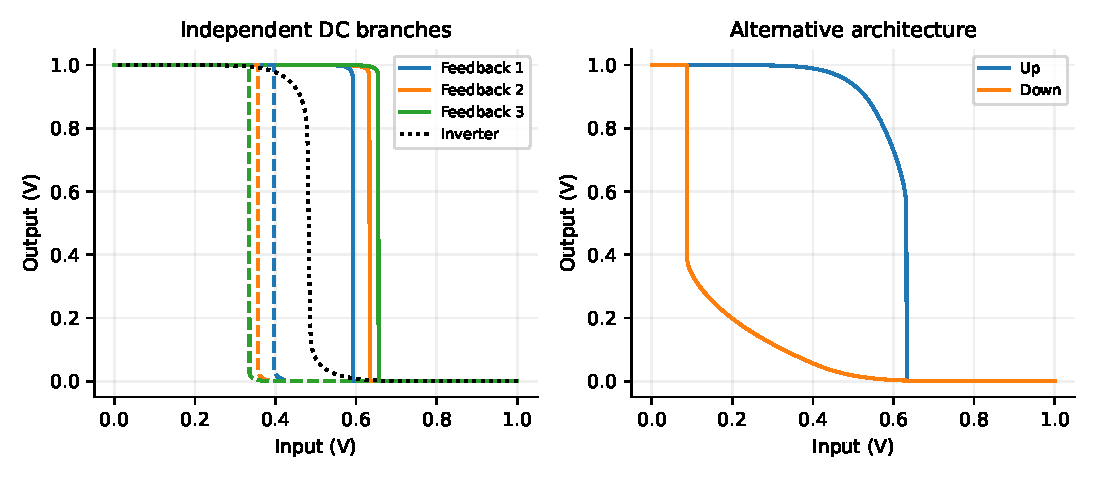
\includegraphics[width=\linewidth]{figures/schmitt_hysteresis.pdf}
\caption{Independent DC hysteresis for three feedback strengths and the alternative; redrawn from this run's HSPICE data.}
\end{figure}
\begin{center}\small
\begin{tabular}{lllll}
\toprule
Circuit & $t_r$ (ps) & $t_f$ (ps) & $t_{pHL}$ (ps) & $t_{pLH}$ (ps) \\
\midrule
INV & 106.95 & 51.92 & 63.86 & 88.77 \\
SCH 1 & 219.10 & 84.35 & 149.36 & 203.59 \\
SCH 2 & 260.52 & 101.05 & 196.67 & 230.75 \\
SCH 3 & 301.50 & 118.33 & 244.97 & 256.13 \\
Alt & 427.75 & 106.61 & 70.70 & 311.56 \\
\bottomrule
\end{tabular}
\end{center}

\begin{figure}[htbp]
\centering
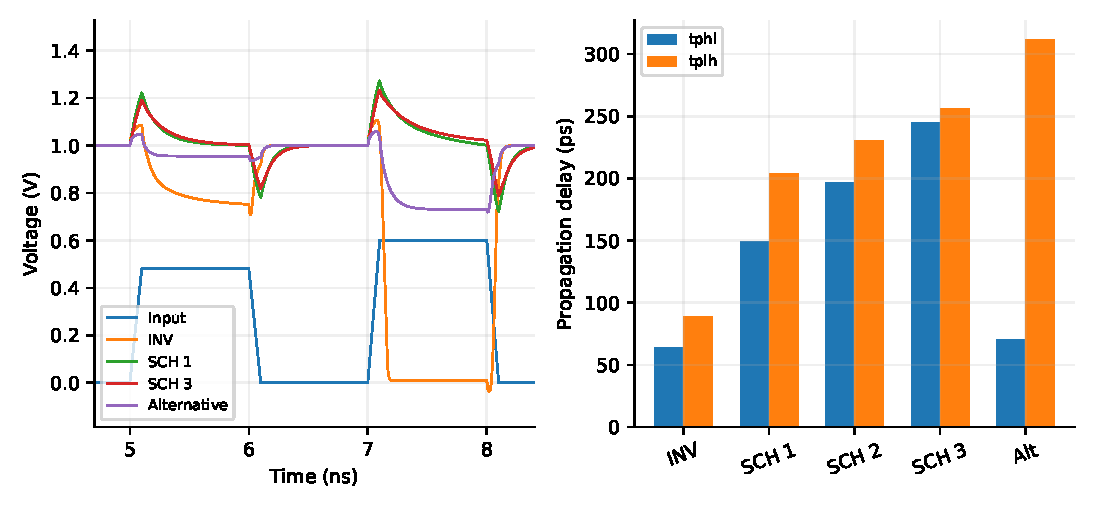
\includegraphics[width=\linewidth]{figures/schmitt_noise_delay.pdf}
\caption{Finite-duration noise and propagation delays with equal loads; redrawn from this run's HSPICE data.}
\end{figure}


\section{Discussion}
Stronger feedback increases DC hysteresis from about 0.195 to 0.320 V while increasing delay. The slower-ramp thresholds differ from independent DC by at most about 1.5 mV, a finite-speed and numerical check rather than proof of the zero-rate limit. A 0.6 V, 0.9 ns disturbance can switch the inverter while the Schmitt retains state during that interval. A short pulse near the DC threshold may not allow regeneration to finish; this does not establish a DC margin beyond the measured threshold. Actual data include temporary rail excursions whose reliability is unverified.

The alternative has about 0.544 V hysteresis but a falling-input threshold near 0.088 V, giving asymmetric noise behavior and a slower rising output. Larger hysteresis is therefore not universally better. Feedback strength must be evaluated together with speed, recovery conditions and input loading.

\section{Conclusion}
All three steps and the alternative-topology question have DC, transient and numerical cross-checks. The speed cost of stronger feedback and asymmetry of the alternative are explicit. Original-process voltage values and unverified reliability limits are not declared satisfied.
